% ----------------------------------------
% LaTeX Article Template for CUED Reports by Jon Sowman, 2009 (jon@hexoc.com)
% ----------------------------------------

\documentclass[12pt]{article} % Set up the document class for an article
\usepackage[margin=2.5cm]{geometry}
%\usepackage{savetrees}		% Concise layout
\usepackage{amssymb}		% This packages permits using $ \therefore $
\usepackage{graphicx}		% SVG graphics includes, amongst other things
\usepackage{epstopdf}		% Allows EPS graphics includes
\usepackage{amsmath}		% This package allows the use of $ \text{} $
\usepackage{placeins}		% This package allows the use of \FloatBarrier
\usepackage{caption}		% This package allows subfigures:
\usepackage{subcaption}	% And proper subfigure captioning
\usepackage{appendix}

\title {\textsc{emission}\\\large{\textsc{The Grid}}}
\author{David Turner (david@dwt27.co.uk)\\Adam Greig (adam@adamgreig.com)}
%\date{} %Suppress date

% Begin the document
\begin{document}
    \maketitle

\begin{abstract}
An art/engineering installation consisting a grid of poles illuminated by white LED strips.  Interactivity is provided through a Computer Vision system utilising a night vision camera.  Applications include display patterns and a virtual ``maze''.
\end{abstract}

\section{Summary of Requirements}
\begin{itemize}
    \item $18m \times 14m$ of unlit ground which can have cables dug in
    \item Mains power, $1.5kW$ peak usage.
\end{itemize}

\section{Design}
\subsection{Layout}
\textsc{The Grid} would occupy a space of approximately $18m \times 14m$.  Of this, $12m \times 12m$ is the grid itself, consisting of a $7 \times 7$ grid of poles with $2m$ spacing.  A backstage area holds the power and control tent as well as the camera mast.

\begin{figure}[h]
    \centering
    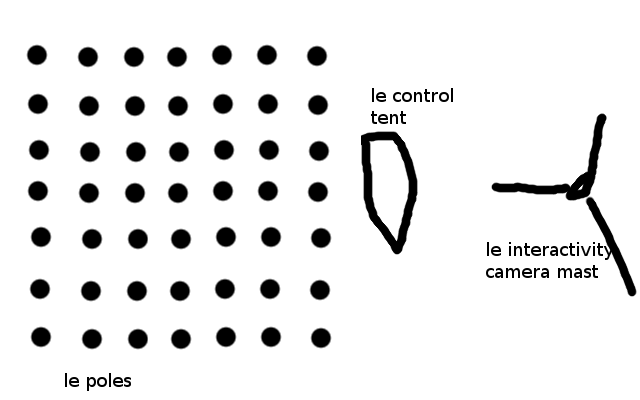
\includegraphics[width=7cm]{diags/plan.png}
    \caption{Plan schematic}
    \label{fig:planschematic}
\end{figure}

\subsection{Structural}
Each pole will protrude $2.5m$ from the ground.  The total length is $3m$, with $50cm$ being inserted into the ground.  The poles are constructed from $\frac{3}{4}" \times \frac{3}{4}" \times \frac{1}{16}"$ aluminium angle section.  See Appendix \ref{app:engdrawings} for detailed drawings.

The interactivity camera will be mounted $8m$ above the ground on a $10m$ fishing pole, guyed for rigidity.

\subsection{Electrical and Electronics}
\subsubsection{Cabling}
Each LED strip will consume around $2A$ when active.  The wiring for one strip will consist of twin core cable carrying power and return between the strip and the control tent.  Additionally, a coaxial connection will run from the interactivity camera to the control tent.

All cabling inside \textsc{The Grid} will be buried slightly below ground to avoid a trip hazard.

\subsubsection{Switching}
Each LED strip will be controlled using a BD679 Darlington pair as a driver.  The drivers will be switched by six 8-output shift registers, themselves controlled by the CPU.

\subsubsection{Power}
The maximum power consumption of \textsc{The Grid} will be $100A$.  This will be provided by four $550W$ ATX power supplies, each rated for $32A$ on the $+12V$ rail.

\subsection{Software and Control}
A laptop in the control tent will generate display patterns and handle interactivity.  It will transmit lighting data via a serial link to an Arduino.  Upon receiving each frame, the Arduino will clock the data into the shift registers, then activate the output latch.

\clearpage
\begin{appendices}
\section{Engineering Drawings}
\label{app:engdrawings}

\begin{figure}[h]
    \centering
    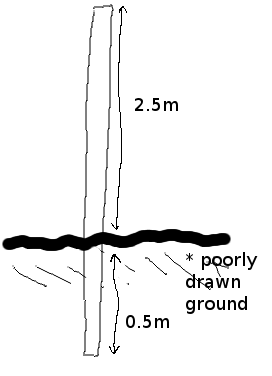
\includegraphics[width=5cm]{diags/sidepole.png}
    \caption{Side view of a single pole}
\end{figure}

\begin{figure}[h]
    \centering
    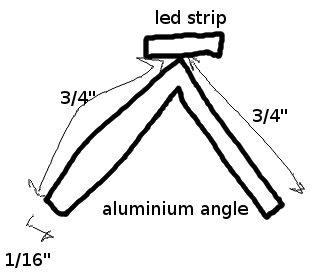
\includegraphics[width=5cm]{diags/toppole.png}
    \caption{Top view of a single pole with LED strip}
\end{figure}

\end{appendices}

\end{document}

